%
% main.tex -- Paper zum Thema <schwimmen>
%
% (c) 2020 Autor, OST Ostschweizer Fachhochschule
%
% !TEX root = ../../buch.tex
% !TEX encoding = UTF-8
%
\chapter{Thema\label{chapter:schwimmen}}
\kopflinks{Thema}
\begin{refsection}
\chapterauthor{Hans Muster}

Ein paar Hinweise für die korrekte Formatierung des Textes
\begin{itemize}
\item
Absätze werden gebildet, indem man eine Leerzeile einfügt.
Die Verwendung von \verb+\\+ ist nur in Tabellen und Arrays gestattet.
\item
Die explizite Platzierung von Bildern ist nicht erlaubt, entsprechende
Optionen werden gelöscht. 
Verwenden Sie Labels und Verweise, um auf Bilder hinzuweisen.
\item
Beginnen Sie jeden Satz auf einer neuen Zeile. 
Damit ermöglichen Sie dem Versionsverwaltungssysteme, Änderungen
in verschiedenen Sätzen von verschiedenen Autoren ohne Konflikt 
anzuwenden.
\item 
Bilden Sie auch für Formeln kurze Zeilen, einerseits der besseren
Übersicht wegen, aber auch um GIT die Arbeit zu erleichtern.
\end{itemize}

%
% einleitung.tex -- Beispiel-File für die Einleitung
%
% (c) 2020 Prof Dr Andreas Müller, Hochschule Rapperswil
%
% !TEX root = ../../buch.tex
% !TEX encoding = UTF-8
%
\section{Teil 0\label{000template:section:teil0}}
\kopfrechts{Teil 0}
Lorem ipsum dolor sit amet, consetetur sadipscing elitr, sed diam
nonumy eirmod tempor invidunt ut labore et dolore magna aliquyam
erat, sed diam voluptua \cite{000template:bibtex}.
At vero eos et accusam et justo duo dolores et ea rebum.
Stet clita kasd gubergren, no sea takimata sanctus est Lorem ipsum
dolor sit amet.

Lorem ipsum dolor sit amet, consetetur sadipscing elitr, sed diam
nonumy eirmod tempor invidunt ut labore et dolore magna aliquyam
erat, sed diam voluptua.
At vero eos et accusam et justo duo dolores et ea rebum.  Stet clita
kasd gubergren, no sea takimata sanctus est Lorem ipsum dolor sit
amet.



%
% teil1.tex -- Beispiel-File für das Paper
%
% (c) 2020 Prof Dr Andreas Müller, Hochschule Rapperswil
%
% !TEX root = ../../buch.tex
% !TEX encoding = UTF-8
%
\section{Teil 1
\label{beispiel:section:teil1}}
\rhead{Problemstellung}
Sed ut perspiciatis unde omnis iste natus error sit voluptatem
accusantium doloremque laudantium, totam rem aperiam, eaque ipsa
quae ab illo inventore veritatis et quasi architecto beatae vitae
dicta sunt explicabo.
Nemo enim ipsam voluptatem quia voluptas sit aspernatur aut odit
aut fugit, sed quia consequuntur magni dolores eos qui ratione
voluptatem sequi nesciunt
\begin{equation}
\int_a^b x^2\, dx
=
\left[ \frac13 x^3 \right]_a^b
=
\frac{b^3-a^3}3.
\label{beispiel:equation1}
\end{equation}
Neque porro quisquam est, qui dolorem ipsum quia dolor sit amet,
consectetur, adipisci velit, sed quia non numquam eius modi tempora
incidunt ut labore et dolore magnam aliquam quaerat voluptatem.

Ut enim ad minima veniam, quis nostrum exercitationem ullam corporis
suscipit laboriosam, nisi ut aliquid ex ea commodi consequatur?
Quis autem vel eum iure reprehenderit qui in ea voluptate velit
esse quam nihil molestiae consequatur, vel illum qui dolorem eum
fugiat quo voluptas nulla pariatur?

\subsection{De finibus bonorum et malorum
\label{beispiel:subsection:finibus}}
At vero eos et accusamus et iusto odio dignissimos ducimus qui
blanditiis praesentium voluptatum deleniti atque corrupti quos
dolores et quas molestias excepturi sint occaecati cupiditate non
provident, similique sunt in culpa qui officia deserunt mollitia
animi, id est laborum et dolorum fuga \eqref{beispiel:equation1}.

Et harum quidem rerum facilis est et expedita distinctio
\ref{beispiel:section:teil2}.
Nam libero tempore, cum soluta nobis est eligendi optio cumque nihil
impedit quo minus id quod maxime placeat facere possimus, omnis
voluptas assumenda est, omnis dolor repellendus
\ref{beispiel:section:teil3}.
Temporibus autem quibusdam et aut officiis debitis aut rerum
necessitatibus saepe eveniet ut et voluptates repudiandae sint et
molestiae non recusandae.
Itaque earum rerum hic tenetur a sapiente delectus, ut aut reiciendis
voluptatibus maiores alias consequatur aut perferendis doloribus
asperiores repellat.



%
% teil2.tex -- Beispiel-File für teil2 
%
% (c) 2020 Prof Dr Andreas Müller, Hochschule Rapperswil
%
% !TEX root = ../../buch.tex
% !TEX encoding = UTF-8
%
\section{Einfacher Bruteforce Algorithmus
  \label{variationsprinzip_algorithmen:section:bruteforce}}
\rhead{Einfacher Bruteforce Algorithmus}
In der Bruteforce-Methode wird jede mögliche Variante durchprobiert, 
um die beste Lösung zu finden. Dabei wird systematisch jede mögliche
Route durchlaufen und überprüft, wie lange die Strecke ist.  
Ablauf durchgemacht und überprüft, wie lange die Strecke ist.
Ist die Strecke kürzer als die bisher kürzeste gefundene Route, 
wird diese als neue optimale Lösung gespeichert.

\begin{figure}
    \centering
    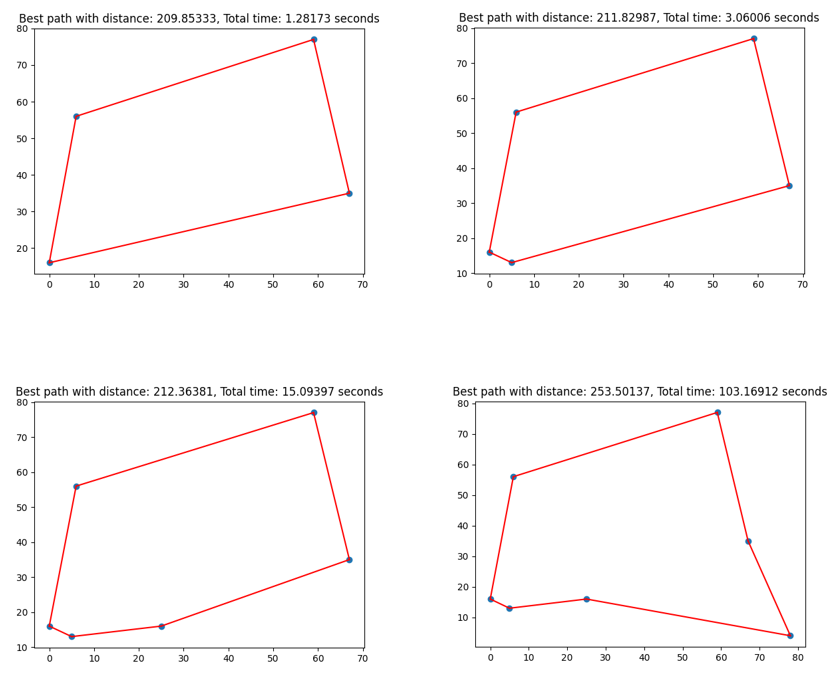
\includegraphics[width=0.8\textwidth]{
        papers/variationsprinzip_algorithmen/images/teil2/02_bruteforce_methode.png
    }
    \caption{Resultate von verschiedener Durchgänge mit steigender Anzahl von Städten}
    \label{fig:results_bruteforce}
\end{figure}

Auf dem Bild \ref{fig:results_bruteforce} ist ersichtlich, dass mit 
jedem weiteren Knoten der Aufwand exponentiell steigt. Anders 
ausgedrückt, mit jeder weiteren Stadt gibt es mehr Varianten, die 
durchprobiert werden müssen. Die Anzahl der Möglichkeiten lässt sich 
mit der Formel

\begin{equation}
    (n-1)!
\end{equation}

berechnen, wobei \(n\) die Anzahl der Städte ist.

Die Berechnung der verschiedenen Kombinationen lässt sich mit folgender 
mathematischen Formel beschreiben:

\begin{equation}
    \label{eq:bruteforce_min_formula}
    L(\sigma) = \sum_{i=1}^{n-1} d(\sigma(i), \sigma(i+1)) + d(\sigma(n), \sigma(1))
\end{equation}

Erklärung:\\
- \( L(\sigma) \)  repräsentiert die Gesamtlänge der Rundreise, die durch 
die Permutation \( \sigma \) der Städte definiert ist.\\
- \( \sigma \) ist eine Permutation der Städte \( \{1, 2, \ldots, n\} \),
wobei jedes \( \sigma \) unterschiedliche Reihenfolge der Städte darstellt.\\
- \( d(i, j) \) ist die Funktion, welche die Entfernung der Stadt \( i \) und 
Stadt \( j \) zurückgibt.\\
- \( L(\sigma) \) die Gesamtlänge der Rundreise \( \sigma \).\\

\subsection{Kurzes Beispiel Rechnung der Formel
    \label{variationsprinzip_algorithmen:section:bruteforce_calculate}}
\rhead{Kurzes Beispiel Rechnung der Formel}
Um zu verdeutlichen, wie die Formel \ref{eq:bruteforce_min_formula}
angewendet wird, folgt hier ein Beispiel.

\begin{table}[h]
    \centering
    \begin{tabular}{|c|c|c|c|c|}
        \hline
          & A  & B  & C  & D  \\ \hline
        A & 0  & 10 & 15 & 20 \\ \hline
        B & 10 & 0  & 35 & 25 \\ \hline
        C & 15 & 35 & 0  & 30 \\ \hline
        D & 20 & 25 & 30 & 0  \\ \hline
    \end{tabular}
    \caption{Beispiel Tabele mit möglicher Distanz der Städten}
    \label{tab:example_bruteforce_cities}
\end{table}

In der Tabelle \ref{tab:example_bruteforce_cities} sind die Distanzen 
zwischen den Städten A, B, C und D aufgeführt. Die Tabelle ist symmetrisch, 
da die Entfernung von Stadt A nach Stadt B gleich der Entfernung von 
Stadt B nach Stadt A ist.
Die Tabelle liesst sich wie folgt: Die Distanz zwischen Stadt B und D 25 beträgt.

Eine mögliche Permutation wäre $\sigma = (A, B, C, D)$ oder $\sigma = (B, D, A, C)$.

Setzt man die Permutation $\sigma = (B, D, A, C)$ in die Formel $\L(\sigma)$
\ref{eq:bruteforce_min_formula} ein, wird die Gesamtdistanz berechnet.


\(i\) und \(i+1\) definiert, welche Position in der Permutation betrachtet wird. 
Beispeil mit \( L(\sigma(1)) \) würde aus dem Set das B genommen und das führt 
dann zu dieser aufstellung
\begin{equation}
    L_1 = d(B, D) + d(D, A) + d(A, C) + d(C, B)
    = 25 + 20 + 15 + 35 = 95
\end{equation}
Dann werden alle möglichen Kombinationen durchgerechnet, und die kürzeste 
Strecke wird als Lösung gewählt.

\subsection{Aufwand Bruteforce
    \label{variationsprinzip_algorithmen:section:bruteforce_efforts}}
\rhead{Aufwand Bruteforce}
Aus den vorherigen Abschnitten ist ersichtlich, dass der Aufwand für die 
Berechnung der kürzesten Strecke exponentiell steigt. Mit jedem weiteren 
Knoten gibt es mehr Variationen, die durchprobiert werden müssen. 

% Tabelle
\begin{table}[ht]
    \centering
    \caption{Zeitverlauf mit steigender Anzahl von Städten}
    \begin{tabular}{cc}
        \toprule
        Punkte & Zeit       \\
        \midrule
        1      & 0,6880     \\
        2      & 0,6905     \\
        3      & 0,7666     \\
        4      & 1,2817     \\
        5      & 3,0601     \\
        6      & 15,0940    \\
        7      & 103,1691   \\
        8      & 1.068,3832 \\
        \bottomrule
    \end{tabular}
\end{table}

%TODO: find out how to make a diagram

Aus der Tabelle und dem Graphen ist ersichtlich, dass der Aufwand mit 
jeder weiteren Stadt exponentiell steigt. Mit 8 Städten dauert die
Berechnung bereits über 17 Minuten.

%
% teil3.tex -- Beispiel-File für Teil 3
%
% (c) 2020 Prof Dr Andreas Müller, Hochschule Rapperswil
%
% !TEX root = ../../buch.tex
% !TEX encoding = UTF-8
%
\section{Teil 3
\label{000template:section:teil3}}
\rhead{Teil 3}
Sed ut perspiciatis unde omnis iste natus error sit voluptatem
accusantium doloremque laudantium, totam rem aperiam, eaque ipsa
quae ab illo inventore veritatis et quasi architecto beatae vitae
dicta sunt explicabo. Nemo enim ipsam voluptatem quia voluptas sit
aspernatur aut odit aut fugit, sed quia consequuntur magni dolores
eos qui ratione voluptatem sequi nesciunt. Neque porro quisquam
est, qui dolorem ipsum quia dolor sit amet, consectetur, adipisci
velit, sed quia non numquam eius modi tempora incidunt ut labore
et dolore magnam aliquam quaerat voluptatem. Ut enim ad minima
veniam, quis nostrum exercitationem ullam corporis suscipit laboriosam,
nisi ut aliquid ex ea commodi consequatur? Quis autem vel eum iure
reprehenderit qui in ea voluptate velit esse quam nihil molestiae
consequatur, vel illum qui dolorem eum fugiat quo voluptas nulla
pariatur?

\subsection{De finibus bonorum et malorum
\label{000template:subsection:malorum}}
At vero eos et accusamus et iusto odio dignissimos ducimus qui
blanditiis praesentium voluptatum deleniti atque corrupti quos
dolores et quas molestias excepturi sint occaecati cupiditate non
provident, similique sunt in culpa qui officia deserunt mollitia
animi, id est laborum et dolorum fuga. Et harum quidem rerum facilis
est et expedita distinctio. Nam libero tempore, cum soluta nobis
est eligendi optio cumque nihil impedit quo minus id quod maxime
placeat facere possimus, omnis voluptas assumenda est, omnis dolor
repellendus. Temporibus autem quibusdam et aut officiis debitis aut
rerum necessitatibus saepe eveniet ut et voluptates repudiandae
sint et molestiae non recusandae. Itaque earum rerum hic tenetur a
sapiente delectus, ut aut reiciendis voluptatibus maiores alias
consequatur aut perferendis doloribus asperiores repellat.




\printbibliography[heading=subbibliography]
\end{refsection}
